\documentclass[12pt,A4]{extarticle}	

\usepackage{amsfonts}
\usepackage{amsmath}
\usepackage{amssymb}
\usepackage{graphicx,wrapfig,lipsum}
\usepackage[german]{babel}
\usepackage{tikz}
\usetikzlibrary{calc, decorations.text}
\usetikzlibrary{decorations.pathreplacing,calligraphy}
\usetikzlibrary{arrows, chains}
\usetikzlibrary{arrows.meta}
\tikzset{>={Latex[width=1.5mm,length=1.5mm]}}


\newcommand{\lectureTitle}{Symmetrische Verschlüsselungsverfahren [unvollständig]}
\newcommand{\semester}{Sommersemester 2023}

\newcommand{\titleSize}{\LARGE}

\usepackage[a4paper,left=0.9cm,right=1cm,top=1.37cm,bottom=2.5cm]{geometry}
\usepackage[utf8]{inputenc}
\usepackage{xifthen}
\usepackage{cmbright}
\usepackage{fontawesome}
\usepackage[T1]{fontenc}
\usepackage{lastpage,lipsum}
\usepackage{hyperref}
\usepackage{transparent}
\usepackage{color}
\usepackage{fancyhdr}

\renewcommand*\familydefault{\sfdefault}
\setlength{\parindent}{0mm}

\definecolor{headerBg}{RGB}{11, 67, 158}
\definecolor{headerGrayColor}{RGB}{210, 210, 210}

\newcommand{\printTitle}{\textcolor{white}{\lectureTitle}\normalsize}
\newcommand{\printSubtitle}{
  \ifdefined\lectureSubtitle
    \textcolor{white}{\small{\lectureSubtitle}}\\
  \fi
}

\fancyhf{}
\pagestyle{fancy}
\fancyhead[C]{
  \fcolorbox{headerBg}{headerBg}{
    \hspace{0.6cm}\begin{minipage}[c][50pt][c]{\paperwidth}
      \begin{minipage}[c]{.7\textwidth}
        \ifdefined\titleSize
          \titleSize \printTitle\\
        \else
          \huge\printTitle\\
        \fi
        \printSubtitle
        \textcolor{headerGrayColor}{\small{\semester}}
      \end{minipage}%
      \begin{minipage}[c]{.2\textwidth}
        \raggedleft
        \textcolor{white}{
          \small{\href{mailto:mail@nilslambertz.de}{\textcolor{white}{\faicon{envelope}} mail@nilslambertz.de}}\\
          \href{https://github.com/nilslambertz/kit-zusammenfassungen}{\textcolor{white}{\faicon{github}} \small{nilslambertz}}}
      \end{minipage}
    \end{minipage}}
}
\renewcommand{\headrulewidth}{0pt}
\setlength{\headheight}{40pt}

\newlength{\oddmarginwidth}
\setlength{\oddmarginwidth}{1in+\hoffset+\oddsidemargin}
\newlength{\evenmarginwidth}
\setlength{\evenmarginwidth}{\evensidemargin+1in}
\fancyhfoffset[LO,RE]{\oddmarginwidth}
\fancyhfoffset[LE,RO]{\evenmarginwidth}
\cfoot{\thepage\ $/$ \pageref*{LastPage}}

\definecolor{highlightColor}{RGB}{66, 135, 245}
\newcommand{\highlight}[1]{\textcolor{highlightColor}{\textbf{#1}}}

\definecolor{noticeColor}{RGB}{235, 110, 38}
\newcommand{\notice}[1]{\textcolor{noticeColor}{#1}}

\newcommand{\redBold}[1]{\textcolor{red}{\textbf{#1}}}

\def\contentsname{\empty}
\addto\captionsgerman{
  \renewcommand{\contentsname}{\empty}
}

\begin{document}

\disclaimer

\tableofcontents
\clearpage

\section{Einführung}
\subsection{Ausgangspunkte für Angriffe}
Angriffe können nach den zur Verfügung stehenden Informationen unterteilt werden:
\begin{itemize}
  \item{\highlight{Ciphertext-Only-Attack}: Nur das \textit{Chiffre}, also die verschlüsselte Nachricht, ist bekannt}
  \item{\highlight{Known-Plaintext-Attack}: Es gibt bekannte Klartext-Chiffre-Paare. Hilfreich sind bekannte Anfangs- und Endphrasen, die in mehreren Nachrichten vorkommen.}
  \item{\highlight{Chosen-Plaintext-Attack}: Es besteht die Möglichkeit, beliebige Texte zu verschlüsseln und somit Klartext-Chiffre-Paare zu erzeugen.}
\end{itemize}

\subsection{Angriffsarten}
\begin{itemize}
  \item{Brute-Force (z.B. alle Schlüssel ausprobieren)}
  \item{Statistische Methoden (z.B. Häufigkeitsanalysen von Buchstaben)}
  \item{Strukturelle Angriffe (z.B. Lineare Kryptoanalyse)}
\end{itemize}

\subsection{Historische Verschlüsselungsverfahren}
Historisch wurden zur Verschlüsselung zwei grundlegende Operationen verwendet:
\begin{itemize}
  \item{\highlight{Substitution}}
  \item{\highlight{Permutation}}
\end{itemize}
Alleine sind beide Verfahren meistens nicht sicher, jedoch verwenden moderne Verschlüsselungsverfahren eine Kombination beider Operationen.

\section{Blockchiffren}
\subsection{Definitionen}
\subsubsection{Definition: Blockchiffre}
Gegeben seien zwei endliche Alphabete $A, B$ und $n, m \in \mathbb{N}$ sowie ein Schlüsselraum $\mathcal{K}$. Eine \highlight{Blockchiffre} ist gegeben durch eine Familie von injektiven Abbildungen $f_k: A^n \rightarrow B^m$ mit $k \in \mathcal{K}$. In der Regel gilt $A = B = \{0, 1\}$ und $n = m$.

\subsubsection{Anforderungen an Blockchiffren}
\begin{itemize}
  \item{Gegeben den Schlüssel $k$ müssen sowohl $f_k$ als auch $f^{-1}_k$ \textbf{effizient} berechenbar sein}
  \item{Ein Angreifer soll nicht zwischen einer \textit{zufälligen Abbildung} und der Blockchiffre mit \textit{zufälligem Schlüssel} unterscheiden können}
\end{itemize}

\subsubsection{Definition: Ideal Cipher}
Eine \highlight{Ideal Cipher} (IC) ist eine (Über-)Idealisierung einer Blockchiffre. Jedem Schlüssel $k \in \{0, 1\}^\lambda$ ist eine vollkommen zufällige Permutation $P_k: \{0, 1\}^n \rightarrow \{0, 1\}^n$ zugeordnet (hierbei sind $\lambda$ und $n$ Sicherheitsparameter) und per Orakelzugriff kann jede Maschine im Modell die Funktionen $P_k$ und $P^{-1}_k$ auswerten. Die Existenz einer solchen IC wird zur Vereinfachung von Beweisen angenommen, man spricht dann von dem \textbf{Ideal-Cipher-Modell}.

\subsubsection{Anforderungen an Ideal Cipher}
\begin{itemize}
  \item{Alle Parteien können über Orakelzugriff $P_k$ und $P^{-1}_k$ auswerten}
  \item{Ideal Cipher liefert zu jedem Paar $(k, m)$ ein $c$ ``zufällig'' gewählt}
  \item{Ideal Cipher liefert zu jedem Paar $(k, c)$ ein $m$ ``zufällig'' gewählt}
  \item{Orakel muss jede Ausgabe speichern, damit für gleiche Nachrichten immer das gleiche Chiffre zurückgegeben wird (nicht parallelisierbar)}
\end{itemize}

\begin{wrapfigure}{r}{9cm}
  \vspace*{-2cm}
  \centering
  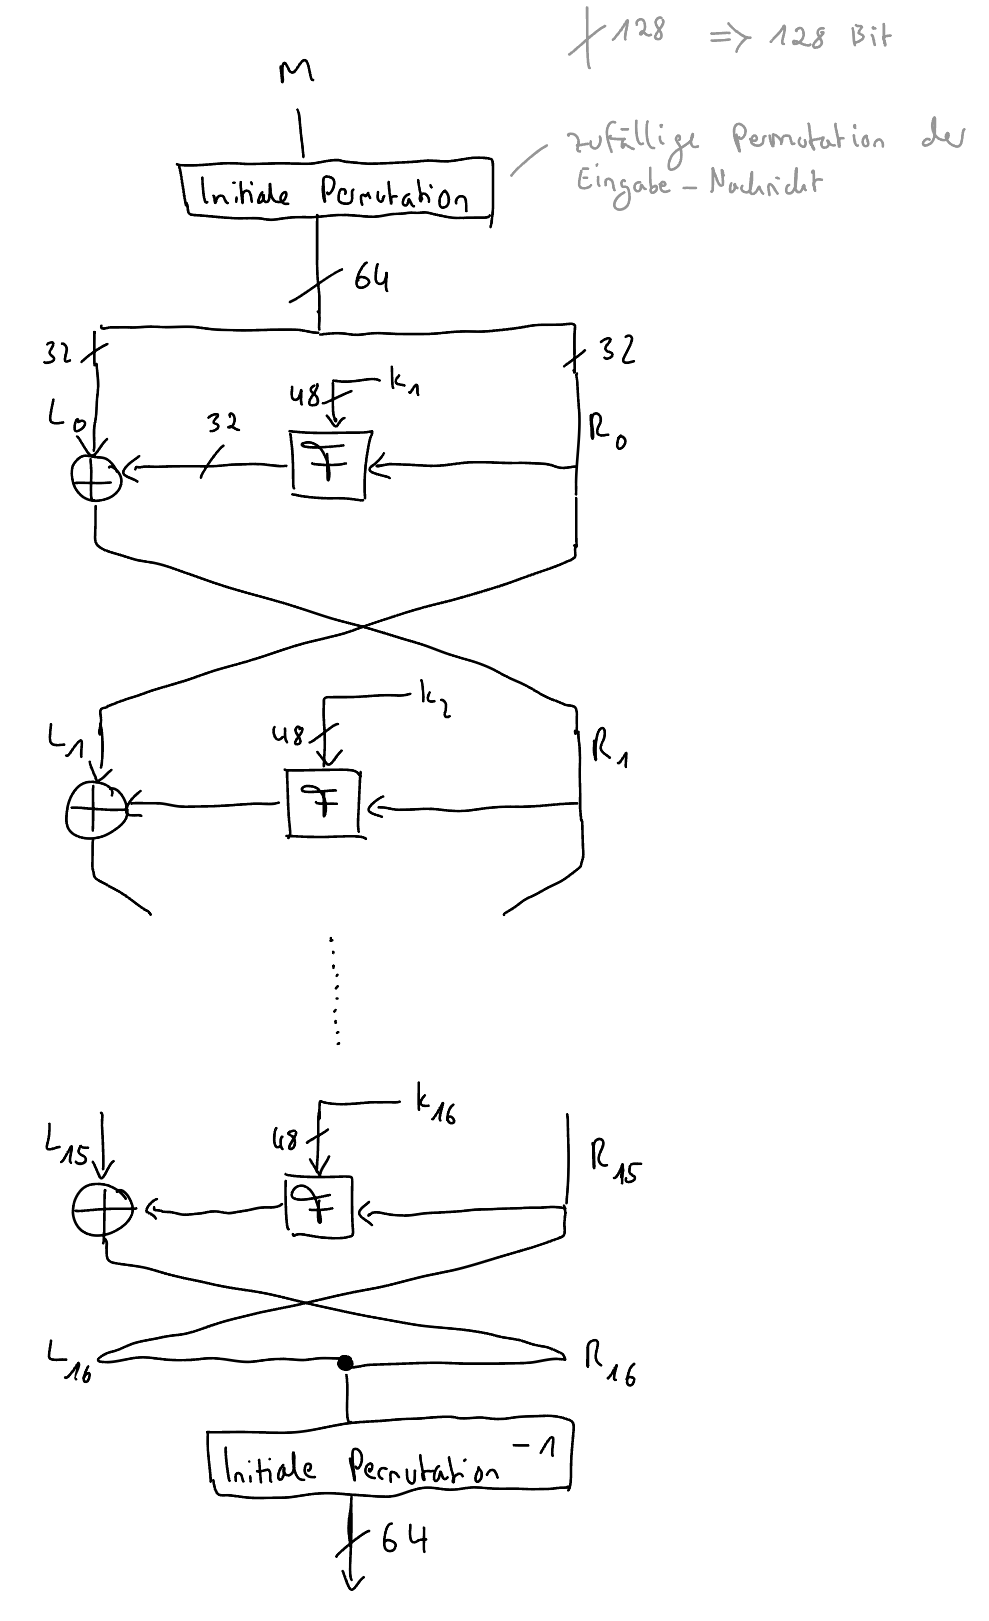
\includegraphics[width=8cm]{../images/des_struktur.png}
  \caption{DES-Verschlüsselungsalgorithmus}
  \vspace*{0.5cm}
  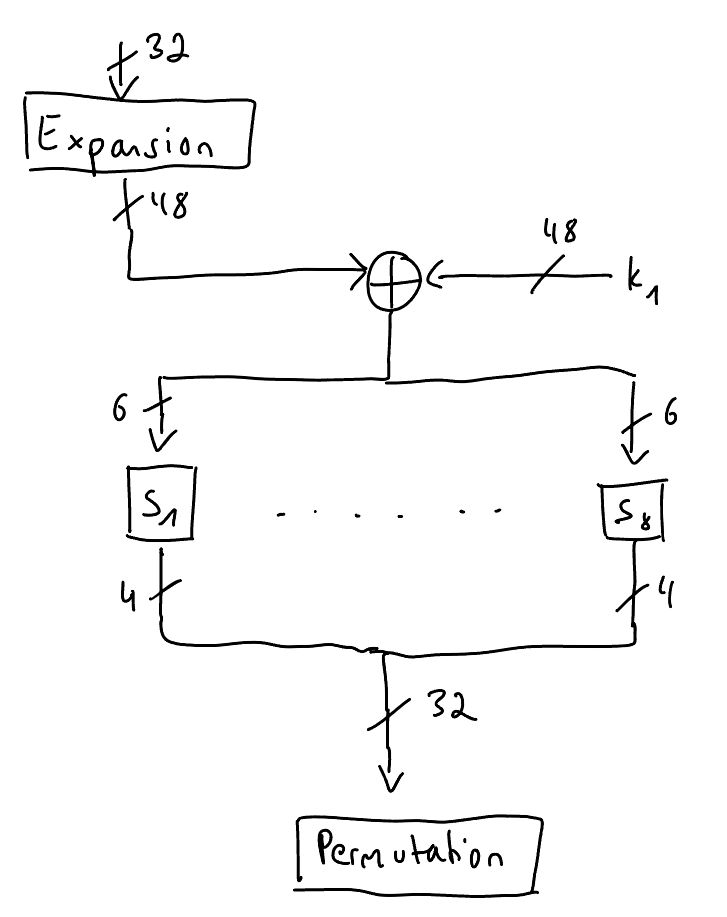
\includegraphics[width=6cm]{../images/des_f_funktion.png}
  \caption{F-Funktion}
  \vspace*{-10cm}
\end{wrapfigure}
\subsection{DES (Data Encryption Standard)}\label{sec:DES}
Der \textbf{Data Encryption Standard} ist eine Blockchiffre mit Schlüssellänge $k = 56$ und Blocklänge $n = 64$, die Verschlüsselungsfunktion ist also $\{0, 1\}^k \times \{0, 1\}^n \rightarrow \{0, 1\}^n$. Er besteht aus einer \textbf{Feistel-Struktur} mit 16 Runden und wurden aufgrund der kurzen Schlüssellänge \textbf{gebrochen}.
\subsubsection{Beispiel für Encryption-Schritt}
$L_1 = R_0$\\
$R_1 = L_0 \oplus F_{k_1}(R_0)$\par
$L_{16} = R_{15}$\\
$R_{16} = L_{15} \oplus F_{k_{16}}(R_{15})$\par

\subsubsection{Beispiel für Decryption-Schritt}
$R_{15} = L_{16}$
\begin{flalign*}
  L_{15} & = R_{16} \oplus F_{k_{16}}(R_{15}) & \\
         & = R_{16} \oplus F_{k_{16}}(L_{16})
\end{flalign*}

\subsubsection{F-Funktion}
Die \highlight{F-Funktion} ist eine nicht-reversible Funktion, die in jeder Runde der Feistel-Struktur ausgeführt wird. Der Ablauf ist folgender:
\begin{enumerate}
  \item{\textbf{Expansion}: Die 32 Eingabebits werden auf 48 Bits erweitert}
  \item{Das bitweise XOR zwischen Expansion und dem Schlüssel wird berechnet}
  \item{Das Ergebnis wird in 6-Bit-Blöcken auf 8 \textbf{Substitutionsboxen} verteilt}
  \item{Die Substitution wird permutiert und ausgeben}
\end{enumerate}

\newpage
\subsection{2DES}\label{sec:2des}
DES wurde aufgrund der kurzen Schlüssellänge (56 Bit) gebrochen und sollte daher nicht mehr in seiner einfachen Form verwendet werden. Es gibt jedoch modifizierte Varianten, die die Sicherheit von DES verbessern, z.B. \textbf{2DES}:\par
Bei 2DES wird die Nachricht zuerst mit $k_1$ verschlüsselt und das Chiffrat dann erneut mit $k_2$ verschlüsselt: $c = DES_{k_2}(DES_{k_1}(m))$

\subsubsection{Angriff auf 2DES}
Gegen 2DES sind \textbf{Meet-in-the-Middle}-Angriffe möglich, dabei wird versucht, die Verschlüsselung von beiden Seiten zu brechen.\par
Gegeben sind zwei Paare $(m_1, c_1)$ und $(m_2, c_2)$, dann funktioniert der Angriff wie folgt:
\begin{enumerate}
  \item{\textbf{Vorwärtsschritt}: Berechne $DES_{k}(m_1)$ und $DES_{k}(m_2)$ für alle $k = 0, \dots, 2^{56} - 1$ und speichere alle Werte in einer Tabelle $T$}
  \item{\textbf{Sortierschritt}: Sortiere Tabelle $T$}
  \item{\textbf{Rückwärtsschritt}: Berechne $DES^{-1}_{k}(c_1)$ und $DES^{-1}_{k}(c_2)$ für alle $k = 0, \dots, 2^{56} - 1$ und suche nach Treffern in $T$}
\end{enumerate}
\underline{\textbf{Zeitaufwand des Angriffs:}}
\begin{enumerate}
  \item{\textbf{Vorwärtsschritt}: $2 * 2^{56}$ DES-Operationen}
  \item{\textbf{Sortierschritt}: $56 * 2^{56}$ Vergleiche}
  \item{\textbf{Rückwärtsschritt}: $2 * 2^{55}$ DES-Operationen (da man nach ungefähr nach der Hälfte fertig ist)}
\end{enumerate}
\underline{\textbf{Speicheraufwand des Angriffs:}}\par
In der Tabelle müssen ungefähr $2^{60}$ Byte gespeichert werden, was ungefähr $1.150.000$ TB entspricht. Damit ist der Angriff so nicht praktikabel.\par
Der Angriff lässt sich ``verbessern'', indem ein Teil des Platzbedarfs mit erhöhtem Rechenaufwand ausgeglichen wird, somit ist das Speicherproblem nicht mehr unüberwindbar, der Angriff dauert aber proportional länger.

\subsection{3DES}
\textbf{3DES} ist analog zu \hyperref[sec:2des]{2DES} definiert. Hierbei werden drei verschiedene Schlüssel $k_1, k_2, k_3$ verwendet. In der mittleren Box wird statt dem normalen $DES$ die inverse Funktion $DES^{-1}$ verwendet. Dadurch kann bei Bedarf $k_1 = k_2 = k_3$ gesetzt werden, wodurch effektiv nur eine $DES$-Verschlüsselung mit $k_1$ ausgeführt wird.\par

\begin{tikzpicture}
  \node (START) at (-2,0) {$m$};
  \node[draw=black, line width=1pt] (A) at (0,0) {$DES$};
  \node[draw=black, line width=1pt] (B) at (3,0) {$DES^{-1}$};
  \node[draw=black, line width=1pt] (C) at (6,0) {$DES$};
  \node (END) at (8,0) {$c$};

  \draw[->] (START) -- (A);
  \draw[->] (A) -- (B);
  \draw[->] (B) -- (C);
  \draw[->] (C) -- (END);

  \draw[->] (0,1) -- (A) node at (0.25, 0.75) {$k_1$};
  \draw[->] (3,1) -- (B) node at (3.25, 0.75) {$k_2$};
  \draw[->] (6,1) -- (C) node at (6.25, 0.75) {$k_3$};
\end{tikzpicture}

\subsubsection{Aufwand für Meet-in-the-Middle-Angriffe gegen 3DES}
\begin{itemize}
  \item{\textbf{Zeit} $\approx 2^{112}$}
  \item{\textbf{Platz} $\approx 2^{56}$}
\end{itemize}

\subsubsection{2Key-3DES}
\textbf{2Key-3DES} ist eine Variation von 3DES, das einen Schlüssel wiederverwendet:\par

\begin{tikzpicture}
  \node (START) at (-2,0) {$m$};
  \node[draw=black, line width=1pt] (A) at (0,0) {$DES$};
  \node[draw=black, line width=1pt] (B) at (3,0) {$DES^{-1}$};
  \node[draw=black, line width=1pt] (C) at (6,0) {$DES$};
  \node (END) at (8,0) {$c$};

  \draw[->] (START) -- (A);
  \draw[->] (A) -- (B);
  \draw[->] (B) -- (C) node at (4.5, 0.25) {$P_j$};
  \draw[->] (C) -- (END);

  \draw[->] (0,1) -- (A) node at (0.25, 0.75) {\redBold{$k_1$}};
  \draw[->] (3,1) -- (B) node at (3.25, 0.75) {$k_2$};
  \draw[->] (6,1) -- (C) node at (6.25, 0.75) {\redBold{$k_1$}};
\end{tikzpicture}

\subsubsection{Advanced Meet-in-the-Middle-Angriff gegen 2Key-3DES}
\begin{enumerate}
  \item{Wähle $0 \dots 0$ als Ergebnis nach erster DES-Box, entschlüssele für alle möglichen Schlüssel: $DES^{-1}_k(0 \dots 0)$\\
              und schreibe Ergebnis in eine Tabelle (die Berechnung liefert sowohl $m$ als auch $P_j$)}
  \item{Lasse alle $2^{56}$ Klartexte $m$ verschlüsseln (chosen-plaintext-attack)}
  \item{Entschlüssele jedes Chiffrat mit \textbf{dem einen} bekannten $k_1$}
  \item{Suche den Wert in der Tabelle, bei Treffern \textit{Kandidat} für $(k_1, k_2)$}
  \item{Überprüfe an weiteren $(m, c)$-Paaren}
\end{enumerate}

\subsubsection{Aufwand für Advanced Meet-in-the-Middle-Angriffe gegen 2Key-3DES}
\begin{itemize}
  \item{\textbf{Zeit} $\approx 3 * 2^{56}$}
  \item{\textbf{Platz} $\approx 2^{56}$}
\end{itemize}

\subsection{Slide-Attacks}
\highlight{Slide-Attacks} sind eine besondere Art von Angriffen, die nur bei Verschlüsselungsverfahren mit besonderer Struktur funktionieren. Die Verschlüsselung muss in mehreren Runden geschehen, wobei in jeder Runde die \textbf{gleiche Funktion} mit \textbf{gleichem Schlüssel} zum verwendet wird.\par
Findet man nun zwei Paare $(m, c)$ und $(m', c')$ wie in der folgenden Grafik, muss nur noch eine Runde gebrochen werden, um den Schlüssel zu erhalten:\par
\begin{tikzpicture}
  \node (START) at (-2,0) {$m$};
  \node[draw=black, line width=1pt] (A) at (0,0) {$f$};
  \node[draw=black, line width=1pt] (B) at (2,0) {$f$};
  \node[draw=black, line width=1pt] (C) at (4,0) {$f$};
  \node (D) at (6,0) {$\dots$};
  \node[draw=black, line width=1pt] (E) at (8,0) {$f$};
  \node[draw=black, line width=1pt] (F) at (10,0) {$f$};
  \node (END) at (12,0) {$c$};

  \draw[->] (START) -- (A);
  \draw[->] (A) -- (B);
  \draw[->] (B) -- (C);
  \draw[->] (C) -- (D);
  \draw[->] (D) -- (E);
  \draw[->] (E) -- (F);
  \draw[->] (F) -- (END);

  \draw[->] (0,1) -- (A) node at (0.25, 0.75) {$k$};
  \draw[->] (2,1) -- (B) node at (2.25, 0.75) {$k$};
  \draw[->] (4,1) -- (C) node at (4.25, 0.75) {$k$};
  \draw[->] (8,1) -- (E) node at (8.25, 0.75) {$k$};
  \draw[->] (10,1) -- (F) node at (10.25, 0.75) {$k$};
\end{tikzpicture}\par
\begin{tikzpicture}
  \hspace{2cm}
  \node (START) at (0,0) {$m'$};
  \node[draw=black, line width=1pt] (A) at (2,0) {$f$};
  \node[draw=black, line width=1pt] (B) at (4,0) {$f$};
  \node[draw=black, line width=1pt] (C) at (6,0) {$f$};
  \node (D) at (8,0) {$\dots$};
  \node[draw=black, line width=1pt] (E) at (10,0) {$f$};
  \node[draw=black, line width=1pt] (F) at (12,0) {$f$};
  \node (END) at (14,0) {$c'$};

  \draw[->] (START) -- (A);
  \draw[->] (A) -- (B);
  \draw[->] (B) -- (C);
  \draw[->] (C) -- (D);
  \draw[->] (D) -- (E);
  \draw[->] (E) -- (F);
  \draw[->] (F) -- (END);

  \draw[->] (2,1) -- (A) node at (2.25, 0.75) {$k$};
  \draw[->] (4,1) -- (B) node at (4.25, 0.75) {$k$};
  \draw[->] (6,1) -- (C) node at (6.25, 0.75) {$k$};
  \draw[->] (10,1) -- (E) node at (10.25, 0.75) {$k$};
  \draw[->] (12,1) -- (F) node at (12.25, 0.75) {$k$};
\end{tikzpicture}

\subsubsection{Zellularautomaten}
Eindimensionale, binäre Zellularautomaten bestehen aus $n$ Zellen, die jeweils ein Bit enthalten.\par
Die Übergangsfunktion $f$ erhält typischerweise $k$ (z.B. 5) Nachbarn (inklusive der Zelle selbst) als Eingabe und gibt als Ergebnis das Bit aus, das im nächsten Schritt an dieser Position steht:\par

\begin{tikzpicture}[
    node distance = 0mm,
    start chain = going right,
    box/.style = {draw, semithick, minimum size=1cm,
        outer sep = 0mm, on chain}
  ]
  \foreach \i [count=\j from 0] in {\dots, \dots, 1, 0, 1, 1, 0, 1, 1, \dots, \dots}
  \node[box] {$\i$};

  \node[label=right:Zeitpunkt $t$] (END) at (12,0) {};

  \draw [thick,decorate,decoration={brace,amplitude=10pt,mirror},yshift=-0.75cm](2.5,0) -- (7.5,0) node[black,midway] {};
\end{tikzpicture}\par
\begin{tikzpicture}[
    node distance = 0mm,
    start chain = going right,
    box/.style = {draw, semithick, minimum size=1cm,
        outer sep = 0mm, on chain}
  ]
  \foreach \i [count=\j from 0] in {\dots, \dots, \dots, \dots, \dots, 1, \dots, \dots, \dots, \dots, \dots}
  \node[box] {$\i$};

  \node[label=right:Zeitpunkt $t+1$] (END) at (12,0) {};
\end{tikzpicture}

\newpage
Die Übergangsfunktion kann auch als Tabelle dargestellt werden:\par
\begin{table}[h]
  \begin{tabular}{c|c}
    Nachbarschaft $N$ & $f(N)$ \\ \hline\hline
    $(0,0,0,0,0)$     & $0$    \\ \hline
    \vdots            & \vdots \\ \hline
    $(0,1,1,0,1)$     & $1$    \\ \hline
    \vdots            & \vdots \\ \hline
    $(1,1,1,1,1)$     & $0$
  \end{tabular}
\end{table}

\subsubsection{Verschlüsselung mit Zellularautomaten}
Um Zellularautomaten als Verschlüsselungsverfahren zu verwenden, müssen sie zudem invertierbar sein, was standardmäßig nicht gegeben ist. Dafür verwenden wir eine Feistel-Struktur, bei dir wir das jedes ``Ergebnis'' $f(N)$ mit dem bisherigen Wert an dieser Stelle XORen:\par
\begin{tikzpicture}[
    node distance = 0mm,
    start chain = going right,
    box/.style = {draw, semithick, minimum size=1cm,
        outer sep = 0mm, on chain}
  ]
  \foreach \i [count=\j from 0] in {\dots, \dots, \dots, \dots, \dots, \notice{1}, \dots, \dots, \dots, \dots, \dots}
  \node[box] {$\i$};

  \node[label=right:Zeitpunkt 0: $IV$] (END) at (12,0) {};
\end{tikzpicture}\par
\begin{tikzpicture}[
    node distance = 0mm,
    start chain = going right,
    box/.style = {draw, semithick, minimum size=1cm,
        outer sep = 0mm, on chain}
  ]
  \foreach \i [count=\j from 0] in {\dots, \dots, 1, 0, 1, 1, 0, 1, 1, \dots, \dots}
  \node[box] {$\i$};

  \node[label=right:Zeitpunkt 1: $m$] (END) at (12,0) {};

  \draw [thick,decorate,decoration={brace,amplitude=10pt,mirror},yshift=-0.75cm](2.5,0) -- (7.5,0) node[black,midway,yshift=-0.75cm] {\notice{1}};
\end{tikzpicture}\par
\begin{tikzpicture}[
    node distance = 0mm,
    start chain = going right,
    box/.style = {draw, semithick, minimum size=1cm,
        outer sep = 0mm, on chain}
  ]
  \foreach \i [count=\j from 0] in {\dots, \dots, \dots, \dots, \dots, \notice{0}, \dots, \dots, \dots, \dots, \dots}
  \node[box] {$\i$};

  \node[label=right:Zeitpunkt 2] (END) at (12,0) {};
  \node (DOTS) at (5,-1) {\vdots};
\end{tikzpicture}\par
\begin{tikzpicture}[
    node distance = 0mm,
    start chain = going right,
    box/.style = {draw, semithick, minimum size=1cm,
        outer sep = 0mm, on chain}
  ]
  \foreach \i [count=\j from 0] in {\dots, \dots, \dots, \dots, \dots, \dots, \dots, \dots, \dots, \dots, \dots}
  \node[box] {$\i$};

  \node[label=right:Zeitpunkt $n$: $c$] (END) at (12,0) {};
\end{tikzpicture}\par
\begin{tikzpicture}[
    node distance = 0mm,
    start chain = going right,
    box/.style = {draw, semithick, minimum size=1cm,
        outer sep = 0mm, on chain}
  ]
  \foreach \i [count=\j from 0] in {\dots, \dots, \dots, \dots, \dots, \dots, \dots, \dots, \dots, \dots, \dots}
  \node[box] {$\i$};

  \node[label=right:Zeitpunkt $n+1$: Zusatzinformation] (END) at (12,0) {};
\end{tikzpicture}\par
Die Zusatzinformation wird benötigt, um zu entschlüsseln.

\subsubsection{Slide-Attack auf Zellularautomaten}
Bei dem Angriff handelt es sich um einen \textbf{Chosen-Plaintext-Angriff}, der wie folgt funktioniert:
\begin{enumerate}
  \item{Setze $m \coloneqq 1 \dots 1$ und $IV \coloneqq 0 \dots 010 \dots 0$ ($IV$ überall 0, außer an einer Stelle)}
  \item{In Zeitpunkt 2 steht damit überall der selbe Wert $a \in \{0, 1\}$, außer an einer Stelle, wo $\neg a$ steht}
  \item{Speichere $m, c$ und $ZI$ (Teil 1)}
  \item{Verschlüssele nun $m' = a \dots a \neg a a \dots a$ (für $a = 0$ und $a = 1$)}
  \item{Bei einem der beiden Fälle erhalten wir als Chiffrat $c'$ (gleich dem Chiffrat aus Teil 1) und $ZI'$}
  \item{Da wir zusätzlich zur Übergangsfunktion XORen, machen wir diese Operation mit $b = c \oplus ZI'$ rückgängig}
  \item{$b$ ist dann das Ergebnis der Übergangsfunktion zum Zeitpunkt $n+1$}
  \item{Damit haben wir Eingaben $c'$ und Ergebnisse $b$ der Übergangsfunktion und können anfangen, die Tabelle zu befüllen}
  \item{Wiederhole das Vorgehen mit anderen $IV$, bis die Tabelle vollständig ist}
  \item{Die fertige Tabelle ist der gesuchte Schlüssel}
\end{enumerate}

\newpage
\textbf{\underline{Visualisierung:}}\par
\begin{tikzpicture}[
    node distance = 0mm,
    start chain = going right,
    box/.style = {draw, semithick, minimum size=1cm,
        outer sep = 0mm, on chain}
  ]
  \foreach \i [count=\j from 0] in {0, 0, 0, 0, 0, 1, 0, 0, 0, 0, 0}
  \node[box] {$\i$};

  \node[label=right:Zeitpunkt 0: $IV$] (END) at (12,0) {};
\end{tikzpicture}\par
\begin{tikzpicture}[
    node distance = 0mm,
    start chain = going right,
    box/.style = {draw, semithick, minimum size=1cm,
        outer sep = 0mm, on chain}
  ]
  \foreach \i [count=\j from 0] in {1, 1, 1, 1, 1, 1, 1, 1, 1, 1, 1}
  \node[box] {$\i$};

  \node[label=right:Zeitpunkt 1: $m$] (END) at (12,0) {};
\end{tikzpicture}\par
\begin{tikzpicture}[
    node distance = 0mm,
    start chain = going right,
    box/.style = {draw, semithick, minimum size=1cm,
        outer sep = 0mm, on chain}
  ]
  \foreach \i [count=\j from 0] in {a, a, a, a, a, \neg a, a, a, a, a, a}
  \node[box] {$\i$};

  \node[label=right:Zeitpunkt 2: $m'$] (END) at (12,0) {};

  \node (DOTS) at (5,-1) {\vdots};
\end{tikzpicture}\par
\begin{tikzpicture}[
    node distance = 0mm,
    start chain = going right,
    box/.style = {draw, semithick, minimum size=1cm,
        outer sep = 0mm, on chain}
  ]
  \foreach \i [count=\j from 0] in {\dots,\dots,\dots,\dots,\dots,\dots,\dots,\dots,\dots,\dots,\dots}
  \node[box] {$\i$};

  \node[label=right:Zeitpunkt $n$: $c$] (END) at (12,0) {};
\end{tikzpicture}\par
\begin{tikzpicture}[
    node distance = 0mm,
    start chain = going right,
    box/.style = {draw, semithick, minimum size=1cm,
        outer sep = 0mm, on chain}
  ]
  \foreach \i [count=\j from 0] in {\dots,\dots,\dots,\dots,\dots,\dots,\dots,\dots,\dots,\dots,\dots}
  \node[box] {$\i$};

  \node[label=right:{Zeitpunkt $n+1$: $ZI = c'$}] (END) at (12,0) {};
\end{tikzpicture}\par
\begin{tikzpicture}[
    node distance = 0mm,
    start chain = going right,
    box/.style = {draw, semithick, minimum size=1cm,
        outer sep = 0mm, on chain}
  ]
  \foreach \i [count=\j from 0] in {\dots,\dots,\dots,\dots,\dots,\dots,\dots,\dots,\dots,\dots,\dots}
  \node[box] {$\i$};

  \node[label=right:{Zeitpunkt $n+2$: $ZI'$}] (END) at (12,0) {};
\end{tikzpicture}

\subsubsection{Advanced Slide-Attack gegen DES-X}
\highlight{DES-X} verwendet DES als Grundlage, arbeitet jedoch zwei Schlüsseln $k_y, k_x$ (jeweils 64-Bit):
\begin{flalign*}
   & c = \text{DES-X}(m) = k_y \oplus \text{DES}_k(m \oplus k_x)            \\
   & m =  \text{DES-X}^{-1}(c) = k_x \oplus \text{DES}^{-1}_k(c \oplus k_y)
\end{flalign*}
Auf den ersten Blick ist nicht klar, wie eine Slide-Attack auf DES-X funktionieren kann, da nichts mehrfach durchgeführt wird. Werden Ver- und Entschlüsselung leicht überlappend aneinandergehangen, kann allerdings ein Angriff konstruiert werden.\par
\begin{wrapfigure}{r}{8.5cm}
  \vspace{-1cm}
  \centering
  \begin{tikzpicture}
    \node (START) at (1,0) {$m$};
    \node (A) at (1,-1) {$\oplus$};
    \node (key-x) at (0,-1) {$k_x$};
    \node[draw=black, line width=1pt] (B) at (1,-2) {$E$};
    \node (key) at (0,-2) {$k$};
    \node (C) at (1,-4) {$\oplus$};
    \node (D) at (1,-5) {$c$};

    \node (E) at (3,-4) {$k_y$};

    \node (F) at (5,-4) {$\oplus$};
    \node[draw=black, line width=1pt] (G) at (5,-6) {$D$};
    \node (key-d) at (4,-6) {$k$};
    \node (H) at (5,-7) {$\oplus$};
    \node (I) at (5,-8) {$m'$};
    \node (key-x-2) at (4,-7) {$k_x$};

    \draw[->] (START) -- (A);
    \draw[->] (key-x) -- (A);
    \draw[->] (key) -- (B);
    \draw[->] (A) -- (B);
    \draw[->] (B) -- (C) node at (1.25, -3) {$c'$};
    \draw[->] (C) -- (D);

    \draw[->] (E) -- (C);
    \draw[->] (E) -- (F);

    \draw[->] (5,-2) -- (F) node at (5.25, -3) {$c'$};
    \draw[->] (F) -- (G) node at (5.25, -5) {$c$};
    \draw[->] (key-d) -- (G);
    \draw[->] (G) -- (H);
    \draw[->] (key-x-2) -- (H);
    \draw[->] (H) -- (I);

  \end{tikzpicture}
  \caption{Konstruktion für den Angriff}
\end{wrapfigure}

\noindent
Was suchen wir überhaupt?
\begin{itemize}
  \item{Wir benötigen ``slid pairs'' $(m,c)$ und $(m', c')$ mit $c \oplus c' = k_y$}
  \item{$m$ erhalten wir durch Zurückrechnen von DES:\begin{flalign*}
                m & = k_x \oplus \text{DES}^{-1}_k(c \oplus k_y) \\
                  & = k_x \oplus \text{DES}^{-1}_k(c')
              \end{flalign*}}
  \item{$m'$ erhalten wir analog:\begin{flalign*}
                m' & = k_x \oplus \text{DES}^{-1}_k(c' \oplus k_y) \\
                   & = k_x \oplus \text{DES}^{-1}_k(c)
              \end{flalign*}}
  \item{Durch Auflösen nach $k_x$ und Gleichsetzen ergibt sich:\begin{flalign*}
                m \oplus \text{DES}^{-1}_k(c'){ }                         & { }= m' \oplus \text{DES}^{-1}_k(c)           \\
                \Leftrightarrow \notice{m \oplus \text{DES}^{-1}_k(c){ }} & \notice{{ }= m' \oplus \text{DES}^{-1}_k(c')} \\
              \end{flalign*}}
  \item{Nun kann der Angriff mit $(m,c)$-Paaren gestartet werden}
\end{itemize}

\newpage
\textbf{Angriff:}\par
Gegeben sind eine Menge von $(m,c)$-Paaren. Für alle ($2^{56}$) Schlüssel $k$:
\begin{enumerate}
  \item{Berechne $m \oplus \text{DES}^{-1}_k(c)$ für alle $(m,c)$-Paare}
  \item{Falls für zwei unterschiedliche Paare $(m, c)$ und $(m',c)$ gilt, dass $m \oplus \text{DES}^{-1}_k(c) = m' \oplus \text{DES}^{-1}_k(c')$, dann sind die Paare ein ``slid pair''-Kandidat}
  \item{Berechne $k_y = c \oplus c'$}
  \item{Berechne damit $k_x = m \oplus \text{DES}^{-1}_k(c \oplus k_y)$}
  \item{Teste $(k, k_x, k_y)$ mit weiteren Paaren auf Korrektheit}
\end{enumerate}

\subsubsection{Aufwand für Advanced Slide-Attack gegen DES-X}
\begin{itemize}
  \item{Mindestens $2^{64 / 2} = 2^{32}$ Klartext-Chiffrat-Paare benötigt ($\approx 32$ GB)}
  \item{Für alle $2^{56}$ Schlüssel: $\approx 2^{32}$ DES-Operationen und Sortieren: $\approx 32 \cdot 2^{32}$}
  \item{Kollision auf Korrektheit prüfen (konstant)}
\end{itemize}
Insgesamt also
\begin{itemize}
  \item{$\approx 2^{88}$ $(= 2^{56} \cdot 2^{32})$ DES-Operationen}
  \item{$\approx 2^{32}$ benötigte $(m,c)$-Paare}
\end{itemize}

\section{Lineare Kryptoanalyse}
Bei der \highlight{Linearen Kryptoanalyse} wird versucht, lineare Abhängigkeiten innerhalb eines Verschlüsselungssystems zu finden (auch wenn diese nur mit einer gewissen Wahrscheinlichkeit auftreten).
\subsection{FEAL-4}
\subsubsection{F-Funktion}

\begin{figure}[h]
  \centering
  \begin{tikzpicture}
    \node[label=left:{$F[0 \dots 7]$}] (F1) at (0,0) {};
    \node[label=left:{$F[8 \dots 15]$}] (F2) at (0,-2) {};
    \node[label=left:{$F[16 \dots 23]$}] (F3) at (0,-4) {};
    \node[label=left:{$F[24 \dots 31]$}] (F4) at (0,-6) {};

    \node[draw=black, line width=1pt] (S0_1) at (2,0) {$S_0$};
    \node[draw=black, line width=1pt] (S1_1) at (6,-2) {$S_1$};
    \node[draw=black, line width=1pt] (S0_2) at (4,-4) {$S_0$};
    \node[draw=black, line width=1pt] (S1_2) at (2,-6) {$S_1$};

    \draw[->] (S0_1) -- (F1);
    \draw[->] (S1_1) -- (F2);
    \draw[->] (S0_2) -- (F3);
    \draw[->] (S1_2) -- (F4);

    \node[label=right:{$B[0 \dots 7]$}] (B1) at (12,0) {};
    \node[label=right:{$B[8 \dots 15]$}] (B2) at (12,-2) {};
    \node[label=right:{$B[16 \dots 23]$}] (B3) at (12,-4) {};
    \node[label=right:{$B[24 \dots 31]$}] (B4) at (12,-6) {};

    \draw[->] (B1) -- (S0_1);
    \draw[->] (B2) -- (S1_1);
    \draw[->] (B3) -- (S0_2);
    \draw[->] (B4) -- (S1_2);

    \node (XOR1) at (8,-2) {\large{$\oplus$}};
    \node (XOR2) at (10,-2) {\large{$\oplus$}};
    \node (XOR3) at (8,-4) {\large{$\oplus$}};
    \node (XOR4) at (10,-4) {\large{$\oplus$}};

    \draw[->] (2,-2) -- (S0_1);
    \draw[->] (4,-2) -- (S0_2);
    \draw[->] (6,-4) -- (S1_1);
    \draw[->] (2,-4) -- (S1_2);

    \draw[->] (10,0) -- (XOR2);
    \draw[->] (10,-6) -- (XOR4);

    \node (k1) at (8,-1) {$k[0 \dots 7]$};
    \node (k2) at (8,-5) {$k[8 \dots 15]$};

    \draw[->] (k1) -- (XOR1);
    \draw[->] (k2) -- (XOR3);
  \end{tikzpicture}
  \caption{$F$-Funktion von FEAL-4}
  \label{feal4_f-function}
\end{figure}
\textbf{FEAL-4} verwendet wie \hyperref[sec:DES]{DES} eine Feistel-Struktur mit einer $F$-Funktion, die in Abbildung \ref{feal4_f-function} dargestellt ist. Die $S$-Boxen führen folgende Berechnung durch:
\begin{flalign*}
  S_i(a,b) \coloneqq rot2((a + b + i) \mod 256)
\end{flalign*}
wobei $rot2$ die Bits um zwei nach links verschiebt (also z.B. $rot2(00000001) = 00000100$).

\subsubsection{Beobachtung}
Die S-Boxen verhalten sich an einer Stelle linear: Das niederwertigste Bit von $(a + b) \mod 256$ entspricht der Summe (dem XOR) der niederwertigsten Bits von $a$ und $b$, da kein Übertrag auftreten kann. Unter Beachtung der Rotation gilt dann
\begin{flalign*}
   & S_0(a,b)[2] = a[0] \oplus b[0]          \\
   & S_1(a,b)[2] = a[0] \oplus b[0] \oplus 1
\end{flalign*}
Damit können wir folgende Gleichungen für das Ergebnis der $F$-Funktion aufstellen:
\begin{flalign*}
   & F[2] = B[0] \oplus F[8]                                                                 \\
   & F[10] = 1 \oplus (B[8] \oplus B[0] \oplus k[0]) \oplus (B[16] \oplus B[24] \oplus k[8])
\end{flalign*}

\begin{wrapfigure}{r}{9cm}
  \centering
  \vspace{1cm}
  \begin{tikzpicture}
    \node(ml) at (0,0) {$m_l$};
    \node(mr) at (6,0) {$m_r$};

    \node (XOR-Start) at (6,-1) {\large{$\oplus$}};
    \node[draw=black, line width=1pt] (F0) at (3,-3) {$F$};
    \node (F0-in) at(6,-3) {};
    \node (XOR0) at (0,-3) {\large{$\oplus$}};
    \node [above right=0cm of F0-in] {$R_0$};
    \node [above left=0cm of XOR0] {$L_0$};
    \draw[->] (ml) -- (XOR0);
    \draw[->] (0,-1) -- (XOR-Start);
    \draw[->] (mr) -- (XOR-Start);
    \draw[->] (6, -3) -- node [midway,above] {$B_0$} (F0);
    \draw[->] (3,-2) -- node [midway,right] {$k_1$} (F0);
    \draw[->] (F0) -- node [midway,above] {$F_0$} (XOR0);
    \draw (XOR-Start) -- (6,-4);
    \draw (XOR0) -- (0,-4);

    \draw (6,-4) -- (0,-5);
    \draw (0,-4) -- (6,-5);
    \node[draw=black, line width=1pt] (F1) at (3,-6) {$F$};
    \node (F1-in) at(6,-6) {};
    \node (XOR1) at (0,-6) {\large{$\oplus$}};
    \node [above right=0cm of F1-in] {$R_1$};
    \node [above left=0cm of XOR1] {$L_1$};
    \draw[->] (0,-5) -- (XOR1);
    \draw[->] (6, -6) -- node [midway,above] {$B_1$} (F1);
    \draw[->] (3,-5) -- node [midway,right] {$k_2$} (F1);
    \draw[->] (F1) -- node [midway,above] {$F_1$} (XOR1);
    \draw (XOR1) -- (0,-7);
    \draw (6,-5) -- (6,-7);

    \draw (6,-7) -- (0,-8);
    \draw (0,-7) -- (6,-8);
    \node[draw=black, line width=1pt] (F2) at (3,-9) {$F$};
    \node (F2-in) at(6,-9) {};
    \node (XOR2) at (0,-9) {\large{$\oplus$}};
    \node [above right=0cm of F2-in] {$R_2$};
    \node [above left=0cm of XOR2] {$L_2$};
    \draw[->] (0,-8) -- (XOR2);
    \draw[->] (6, -9) -- node [midway,above] {$B_2$} (F2);
    \draw[->] (3,-8) -- node [midway,right] {$k_3$} (F2);
    \draw[->] (F2) -- node [midway,above] {$F_2$} (XOR2);
    \draw (XOR2) -- (0,-10);
    \draw (6,-8) -- (6,-10);

    \draw (6,-10) -- (0,-11);
    \draw (0,-10) -- (6,-11);
    \node[draw=black, line width=1pt] (F3) at (3,-12) {$F$};
    \node (F3-in) at(6,-12) {};
    \node (XOR3) at (0,-12) {\large{$\oplus$}};
    \node [above right=0cm of F3-in] {$R_3$};
    \node [above left=0cm of XOR3] {$L_3$};
    \node (XOR-End) at (6,-13) {\large{$\oplus$}};
    \node (cl) at (0,-14) {$c_l$};
    \node (cr) at (6,-14) {$c_r$};
    \draw[->] (0,-11) -- (XOR3);
    \draw[->] (6, -12) -- node [midway,above] {$B_3$} (F3);
    \draw[->] (3,-11) -- node [midway,right] {$k_4$} (F3);
    \draw[->] (F3) -- node [midway,above] {$F_3$} (XOR3);
    \draw[->] (0,-13) -- (XOR-End);
    \draw[->] (6,-11) -- (XOR-End);
    \draw[->] (XOR3) -- (cl);
    \draw[->] (XOR-End) -- (cr);
  \end{tikzpicture}
  \caption{Struktur von FEAL-4 (vereinfacht)}
  \label{feal4}
  \vspace*{-10cm}
\end{wrapfigure}

\noindent
\subsubsection{Charakteristik}
FEAL-4 besteht aus 4 Runden, in denen die $F$-Funktion mit einem 16-Bit-Schlüssel ausgeführt wird (siehe Abbildung \ref{feal4}).
Mithilfe der gerade aufgestellten Gleichungen lassen sich folgende Charakteristiken ableiten:
\begin{flalign*}
  F_0[2,8] & \coloneqq F_0[2] \oplus F_0[8] \\
           & = B_0[0]                       \\ \\
  R_1[2,8] & = F_0[2,8] \oplus m_l[2,8]     \\
           & = B_0[0] \oplus m_l[2,8]       \\
           & = m_l[0,2,8] \oplus m_r[0]     \\ \\
  R_1[2,8] & = F_2[2,8] \oplus R_3[2,8]     \\
           & = B_2[0] \oplus R_3[2,8]       \\
           & = L_3[0] \oplus R_3[2,8]       \\ \\
\end{flalign*}
Durch Gleichsetzen erhalten wir:
\begin{flalign*}
  m_l[0,2,8] \oplus m_r[0] = L_3[0] \oplus R_3[2,8]
\end{flalign*}
Dadurch haben wir eine Beziehung zwischen der Nachricht und dem Ergebnis der vorletzten Runde ($L_3$ und $R_3$) gefunden.

\newpage
\subsubsection{Angriff}\label{sec:feal4-angriff}
Gegeben sind eine Menge von $(m,c)$-Paaren. Für alle ($2^{16}$) Schlüssel $k_4$:
\begin{enumerate}
  \item{Entschlüssele $c$ mit $k_4$, daduch erhalten wir $L_3$ und $R_3$}
  \item{Falls die gefundene Gleichung $m_l[0,2,8] \oplus m_r[0] = L_3[0] \oplus R_3[2,8]$ nicht für alle $(m,c)$-Paare gilt, ist $k_4$ falsch}
  \item{Wiederhole mit verschiedenen Charakteristiken, bis nur noch wenige $k_4$ übrig sind}
  \item{Führe den Angriff analog gegen $k_1$ durch}
  \item{Wenn $k_1$ und $k_4$ bekannt, können $k_2$ und $k_3$ durch vollständige Suche (jeweils $2^{16}$) gefunden werden}
\end{enumerate}

\subsubsection{Aufwand}
\begin{itemize}
  \item{$\approx 16$ (besser $\approx 20$) Klartext-Chiffrat-Paare benötigt}
  \item{Rechenaufwand $\approx 2^{16}$}
\end{itemize}

\subsection{DES}
\subsubsection{Angriff}
Auch bei \hyperref[sec:DES]{DES} ist die lineare Analyse möglich, obwohl die $S$-Boxen (6 Eingänge, 4 Ausgänge) keine linearen Funktionen sind. Bei $S_5$ hat eine lineare Beziehung der Ein- und Ausgänge die Wahrscheinlichkeit $\frac{3}{16} \approx 0.19$.\par
Diese Beziehung lässt sich auf 3 Runden erweitern. Dann kann der Angriff wie bei \hyperref[sec:feal4-angriff]{FEAL-4} durchgeführt werden. Für 16 Runden (wie bei DES üblich) kann auch eine Beziehung gefunden werden, die Erfolgswahrscheinlichkeit sinkt dabei allerdings.\par
\textit{Details zum Angriff im Skript.}

\subsubsection{Aufwand}
\begin{itemize}
  \item{$\approx 2^{47}$ Klartext-Chiffrat-Paare benötigt}
  \item{``Zurückrechnen'' der ersten und letzten Runde nur $2 \cdot 2^6$ (liefert 14 Bit des Schlüssels)}
  \item{Restliche 42 Bit des Schlüssels müssen durch vollständige Suche gefunden werden}
  \item{Schneller als Brute-Force ($2^{56}$), aber sehr viele  Klartext-Chiffrat-Paare benötigt}
\end{itemize}

\section{Differentielle Kryptoanalyse}
Bei der \highlight{Differentiellen Kryptoanalyse} werden Differenzen zwischen Klartexten betrachtet (meistens per XOR), welche mit einer gewissen Wahrscheinlichkeit zu bestimmten Differenzen in den zugehörigen Chiffraten führen.

\subsection{DES}
\subsubsection{Idee}
Wir betrachten nun nicht mehr $(m, c)$-Paare, sondern zwei Paare $(m_1, c_1), (m_2, c_2)$ und deren Differenz $(m', c')$ mit $m' \coloneqq m_1 \oplus m_2$ und $c' \coloneqq c_1 \oplus c_2$.\par
Da der Schlüssel nur per XOR eingeht und sich dadurch die Differenzen der Zwischenergebnisse nicht ändern, können dadurch Informationen über den Schlüssel gewonnen werden.

\newpage
\begin{figure}[h]
  \centering
  \begin{tikzpicture}
    \node(m) at (0,0) {$m_1$};
    \node[draw=black, line width=1pt] (Exp) at (0,-1) {$Erw.$};
    \node (k) at (1,-3) {$k$};
    \node (XOR) at (0,-3) {\large{$\oplus$}};
    \node[draw=black, line width=1pt] (S) at (0,-5) {$S$};
    \node(End) at (0,-7) {};
    \draw[->] (m) -- (Exp);
    \draw[->] (Exp) -- node [midway,right] {$e_1$} (XOR);
    \draw[->] (k) -- (XOR);
    \draw[->] (XOR) -- node [midway,right] {$s_{\text{in},1} = e_1 \oplus k$} (S);
    \draw[->] (S) -- node [midway,right] {$s_{\text{out},1}$} (End);
  \end{tikzpicture}
  \hspace{1.5cm}
  \begin{tikzpicture}
    \node(m) at (0,0) {$m_2$};
    \node[draw=black, line width=1pt] (Exp) at (0,-1) {$Erw.$};
    \node (k) at (1,-3) {$k$};
    \node (XOR) at (0,-3) {\large{$\oplus$}};
    \node[draw=black, line width=1pt] (S) at (0,-5) {$S$};
    \node(End) at (0,-7) {};
    \draw[->] (m) -- (Exp);
    \draw[->] (Exp) -- node [midway,right] {$e_2$} (XOR);
    \draw[->] (k) -- (XOR);
    \draw[->] (XOR) -- node [midway,right] {$s_{\text{in},2} = e_2 \oplus k$} (S);
    \draw[->] (S) -- node [midway,right] {$s_{\text{out},2}$} (End);
  \end{tikzpicture}
  \hspace{1.5cm}
  \begin{tikzpicture}
    \node(m) at (0,0) {$m' = m_1 \oplus m_2$};
    \node[draw=black, line width=1pt] (Exp) at (0,-1) {$Erw.$};
    \node (NO-XOR) at (0,-3) {};
    \node[draw=black, line width=1pt] (S) at (0,-5) {$S$};
    \node(End) at (0,-7) {};
    \draw[->] (m) -- (Exp);
    \draw[->] (Exp) -- (S);
    \draw(Exp) -- node [midway,right] {$e' = e_1 \oplus e_2 = Erw.(m')$} (NO-XOR);
    \draw (NO-XOR) -- node [midway,right] {$s'_{\text{in}} = e'$} (S);
    \draw[->] (S) -- node [midway,right] {$s'_{\text{out}} = s_{\text{out},1} \oplus s_{\text{out},2}$} (End);
  \end{tikzpicture}
  \caption{DES-$S$-Boxen und Zwischenergebnisse mit Eingaben und Differenzen}
\end{figure}

\subsubsection{Angriff auf 1-Runden-DES}
\textbf{Beobachtung:} $s'_{\text{in}} = e' = e_1 \oplus e_2$ ist unabhängig von $k$.\par
Wir erstellen uns nun für jede $S$-Box eine \textbf{Differenz-Tabelle}, die alle möglichen Kombinationen von Ein- und Ausgangsdifferenzen enthält ($64 \times 16$-Tabelle). Zeile $i$ entspricht der Eingangsdifferenz $s'_{\text{in}} = i$. In Spalte $j$ sind alle Paare $s_{\text{in},1}$ und $s_{\text{in},2}$ eingetragen, für die die Ausgangsdifferenz $s'_{\text{out}} = j$ ist.
\begin{enumerate}
  \item{Berechne $s'_{\text{in}}$ und $s'_{\text{out}}$ aus $(m_1, c_1)$ und $(m_2, c_2)$}
  \item{Lese mögliche $s_{\text{in},1}$ und $s_{\text{in},2}$ aus der Tabelle ab}
  \item{Berechne alle Schlüsselkandidaten $k$ durch $k = s_{\text{in},1} \oplus e_1$ (gilt, da $s_{\text{in},1} = e_1 \oplus k$)}
  \item{Wiederhole mit anderen Paaren, bis nur noch ein Kandidat $k$ übrig ist}
\end{enumerate}

\end{document}